%============================================================================
% tento soubor pouzijte jako zaklad
% (c) 2008 Michal Bidlo
% E-mail: bidlom AT fit vutbr cz
%============================================================================
% kodovaní: UTF-8 (zmena prikazem iconv, recode nebo cstocs)
%----------------------------------------------------------------------------
% zpracování: make, make pdf, make desky, make clean
%============================================================================
% Šablonu upravil: Ing. Jaroslav Dytrych, idytrych@fit.vutbr.cz
%============================================================================
\documentclass[]{fitthesis} % bez zadání - pro začátek práce, aby nebyl problém s překladem
%\documentclass[zadani]{fitthesis} % odevzdani do wisu - odkazy jsou barevné
%\documentclass[zadani,print]{fitthesis} % pro tisk - odkazy jsou černé
%\documentclass[english,print]{fitthesis} % pro tisk - odkazy jsou černé
% * Je-li prace psana v anglickem jazyce, je zapotrebi u tridy pouzit 
%   parametr english nasledovne:
%      \documentclass[english]{fitthesis}
% * Je-li prace psana ve slovenskem jazyce, je zapotrebi u tridy pouzit 
%   parametr slovak nasledovne:
%      \documentclass[slovak]{fitthesis}

\usepackage[czech,slovak,english]{babel}
\usepackage[T1]{fontenc}
\usepackage[utf8]{inputenc} %kodovani
\usepackage{cmap}
\usepackage{url}
\DeclareUrlCommand\url{\def\UrlLeft{<}\def\UrlRight{>} \urlstyle{tt}}

%zde muzeme vlozit vlastni balicky
\usepackage{listings}
\usepackage[toc,page,header]{appendix}
\RequirePackage{titletoc}
\ifczech
  \usepackage{ae}
\fi
\usepackage{mathtools}
\usepackage[czech,ruled,longend,noline]{algorithm2e}
\usepackage{graphicx}
\usepackage{float}
\usepackage{amsthm}
\usepackage{multirow,tabularx}
\usepackage{booktabs}
\theoremstyle{definition}
\newtheorem{defn}{Definice}[section]


%---rm---------------
\renewcommand{\rmdefault}{lmr}%zavede Latin Modern Roman jako rm
%---sf---------------
\renewcommand{\sfdefault}{qhv}%zavede TeX Gyre Heros jako sf
%---tt------------
\renewcommand{\ttdefault}{lmtt}% zavede Latin Modern tt jako tt

%-----------------------------------------------------------------------------


% Níže jsou deklarace fontů pro testování a ladění JVS 
% - doporučuje se NEPOUŽÍVAT
% Deklarace nejsou doladěné !!!
% Times New Roman není dle JVS povolený (je tu na ukázku)
%-----------------------------------------------------------------------------

\ifOPEN
  \pdfmapfile{=OpenSansfontspdf.map}
  \DeclareFontFamily{T1}{OpenSans}{}
  \DeclareFontShape{T1}{OpenSans}{b}{n}{<->recOpenSans-Bold}{}
  \DeclareFontShape{T1}{OpenSans}{b}{it}{<->recOpenSans-BoldItalic}{}
  \DeclareFontShape{T1}{OpenSans}{eb}{n}{<->recOpenSans-ExtraBold}{}
  \DeclareFontShape{T1}{OpenSans}{eb}{it}{<->recOpenSans-ExtraBoldItalic}{}
  \DeclareFontShape{T1}{OpenSans}{m}{it}{<->recOpenSans-Italic}{}
  \DeclareFontShape{T1}{OpenSans}{l}{n}{<->recOpenSans-Light}{}
  \DeclareFontShape{T1}{OpenSans}{l}{it}{<->recOpenSans-LightItalic}{}
  \DeclareFontShape{T1}{OpenSans}{m}{n}{<->recOpenSans-Regular}{}
  \DeclareFontShape{T1}{OpenSans}{sb}{n}{<->recOpenSans-Semibold}{}
  \DeclareFontShape{T1}{OpenSans}{sb}{it}{<->recOpenSans-SemiboldItalic}{}
  \renewcommand{\rmdefault}{OpenSans}
  \renewcommand{\sfdefault}{OpenSans}
\else
  \iftoggle{declare_open}{
    \pdfmapfile{=OpenSansfontspdf.map}
    \DeclareFontFamily{T1}{OpenSans}{}
    \DeclareFontShape{T1}{OpenSans}{b}{n}{<->recOpenSans-Bold}{}
    \DeclareFontShape{T1}{OpenSans}{b}{it}{<->recOpenSans-BoldItalic}{}
    \DeclareFontShape{T1}{OpenSans}{eb}{n}{<->recOpenSans-ExtraBold}{}
    \DeclareFontShape{T1}{OpenSans}{eb}{it}{<->recOpenSans-ExtraBoldItalic}{}
    \DeclareFontShape{T1}{OpenSans}{m}{it}{<->recOpenSans-Italic}{}
    \DeclareFontShape{T1}{OpenSans}{l}{n}{<->recOpenSans-Light}{}
    \DeclareFontShape{T1}{OpenSans}{l}{it}{<->recOpenSans-LightItalic}{}
    \DeclareFontShape{T1}{OpenSans}{m}{n}{<->recOpenSans-Regular}{}
    \DeclareFontShape{T1}{OpenSans}{sb}{n}{<->recOpenSans-Semibold}{}
    \DeclareFontShape{T1}{OpenSans}{sb}{it}{<->recOpenSans-SemiboldItalic}{}
  }
\fi


\ifVAFLE
  \pdfmapfile{=Vafle_VUT_fontspdf.map}
  \DeclareFontFamily{T1}{VafleVUT}{}
  \DeclareFontShape{T1}{VafleVUT}{m}{n}{<->recVafle_VUT_Regular}{}
  \DeclareFontShape{T1}{VafleVUT}{b}{n}{<->recVafle_VUT_Bold}{}
  \DeclareFontShape{T1}{VafleVUT}{l}{n}{<->recVafle_VUT_Light}{}
  \renewcommand{\rmdefault}{VafleVUT}
  \renewcommand{\sfdefault}{VafleVUT}
  % Tohle je škaredý hack - Vafle nemá it a když se s tím nic neudělá, kurzíva
  % se nijak neprojeví (jen varováním při překladu). Nicméně "doplňkový" font 
  % OpenSans kurzívu má a v semibold to dle mého názoru vypadá pro demonstrační
  % účely při ladění JVS přijatelně.
  \let\oldit\it
  \renewcommand{\it}{\usefont{T1}{OpenSans}{sb}{it}}
\else
  \ifTVAFLE
    \pdfmapfile{=Vafle_VUT_fontspdf.map}
    \DeclareFontFamily{T1}{VafleVUT}{}
    \DeclareFontShape{T1}{VafleVUT}{m}{n}{<->recVafle_VUT_Regular}{}
    \DeclareFontShape{T1}{VafleVUT}{b}{n}{<->recVafle_VUT_Bold}{}
    \DeclareFontShape{T1}{VafleVUT}{l}{n}{<->recVafle_VUT_Light}{}
    \pdfmapfile{=OpenSansfontspdf.map}
    \DeclareFontFamily{T1}{OpenSans}{}
    \DeclareFontShape{T1}{OpenSans}{b}{n}{<->recOpenSans-Bold}{}
    \DeclareFontShape{T1}{OpenSans}{b}{it}{<->recOpenSans-BoldItalic}{}
    \DeclareFontShape{T1}{OpenSans}{eb}{n}{<->recOpenSans-ExtraBold}{}
    \DeclareFontShape{T1}{OpenSans}{eb}{it}{<->recOpenSans-ExtraBoldItalic}{}
    \DeclareFontShape{T1}{OpenSans}{m}{it}{<->recOpenSans-Italic}{}
    \DeclareFontShape{T1}{OpenSans}{l}{n}{<->recOpenSans-Light}{}
    \DeclareFontShape{T1}{OpenSans}{l}{it}{<->recOpenSans-LightItalic}{}
    \DeclareFontShape{T1}{OpenSans}{m}{n}{<->recOpenSans-Regular}{}
    \DeclareFontShape{T1}{OpenSans}{sb}{n}{<->recOpenSans-Semibold}{}
    \DeclareFontShape{T1}{OpenSans}{sb}{it}{<->recOpenSans-SemiboldItalic}{}
  \fi
\fi

\ifARIAL
  \pdfmapfile{=arialfontspdf.map}
  \DeclareFontFamily{T1}{arial}{}
  \DeclareFontShape{T1}{arial}{b}{n}{<->recarialbd}{}
  \DeclareFontShape{T1}{arial}{b}{sl}{<->recarialbdo}{}
  \DeclareFontShape{T1}{arial}{b}{it}{<->recarialbi}{}
  \DeclareFontShape{T1}{arial}{m}{n}{<->recarial}{}
  \DeclareFontShape{T1}{arial}{m}{sl}{<->recarialo}{}
  \DeclareFontShape{T1}{arial}{m}{it}{<->recariali}{}
  \DeclareFontShape{T1}{arial}{bx}{n}{<->ssub * arial/b/n}{}
  \DeclareFontShape{T1}{arial}{bx}{sl}{<->ssub * arial/b/sl}{}
  \DeclareFontShape{T1}{arial}{bx}{it}{<->ssub * arial/b/it}{}
  \renewcommand{\rmdefault}{arial}
  \renewcommand{\sfdefault}{arial}
\else
  \ifTARIAL
    \pdfmapfile{=arialfontspdf.map}
    \DeclareFontFamily{T1}{arial}{}
    \DeclareFontShape{T1}{arial}{b}{n}{<->recarialbd}{}
    \DeclareFontShape{T1}{arial}{b}{sl}{<->recarialbdo}{}
    \DeclareFontShape{T1}{arial}{b}{it}{<->recarialbi}{}
    \DeclareFontShape{T1}{arial}{m}{n}{<->recarial}{}
    \DeclareFontShape{T1}{arial}{m}{sl}{<->recarialo}{}
    \DeclareFontShape{T1}{arial}{m}{it}{<->recariali}{}
    \DeclareFontShape{T1}{arial}{bx}{n}{<->ssub * arial/b/n}{}
    \DeclareFontShape{T1}{arial}{bx}{sl}{<->ssub * arial/b/sl}{}
    \DeclareFontShape{T1}{arial}{bx}{it}{<->ssub * arial/b/it}{}
  \fi
\fi

\ifTIMES
  \pdfmapfile{=timesfontspdf.map}
  \DeclareFontFamily{T1}{times}{}
  \DeclareFontShape{T1}{times}{m}{n}{<->rectimes}{}
  \DeclareFontShape{T1}{times}{m}{it}{<->rectimesi}{}
  \DeclareFontShape{T1}{times}{b}{n}{<->rectimesbd}{}
  \DeclareFontShape{T1}{times}{b}{it}{<->rectimesbi}{}
  \renewcommand{\rmdefault}{times}
  \renewcommand{\sfdefault}{times}
\fi


% vypne funkci nové šablony, která automaticky nahrazuje uvozovky,
% aby nebyly prováděny nevhodné náhrady v popisech API apod.
\csdoublequotesoff

% =======================================================================
% balíček "hyperref" vytváří klikací odkazy v pdf, pokud tedy použijeme pdflatex
% problém je, že balíček hyperref musí být uveden jako poslední, takže nemůže
% být v šabloně
\ifWis
\ifx\pdfoutput\undefined % nejedeme pod pdflatexem
\else
  \usepackage{color}
  \usepackage[unicode,colorlinks,hyperindex,plainpages=false,pdftex]{hyperref}
  \definecolor{links}{rgb}{0.4,0.5,0}
  \definecolor{anchors}{rgb}{1,0,0}
  \def\AnchorColor{anchors}
  \def\LinkColor{links}
  \def\pdfBorderAttrs{/Border [0 0 0] }  % bez okrajů kolem odkazů
  \pdfcompresslevel=9
\fi
\else % pro tisk budou odkazy, na které se dá klikat, černé
\ifx\pdfoutput\undefined % nejedeme pod pdflatexem
\else
  \usepackage{color}
  \usepackage[unicode,colorlinks,hyperindex,plainpages=false,pdftex,urlcolor=black,linkcolor=black,citecolor=black]{hyperref}
  \definecolor{links}{rgb}{0,0,0}
  \definecolor{anchors}{rgb}{0,0,0}
  \def\AnchorColor{anchors}
  \def\LinkColor{links}
  \def\pdfBorderAttrs{/Border [0 0 0] } % bez okrajů kolem odkazů
  \pdfcompresslevel=9
\fi
\fi

%Informace o praci/projektu
%---------------------------------------------------------------------------
\projectinfo{
  %Prace
  project=BP,            %typ prace BP/SP/DP/DR
  year=2016,             %rok
  date=\today,           %datum odevzdani
  %Nazev prace
  title.cs={Obnova hesel archivů ZIP s~využitím GPU},  %nazev prace v cestine ci slovenstine
  title.en={Password Recovery of ZIP Archives Using GPU}, %nazev prace v anglictine
  %Autor
  author={Vojtěch Večeřa},   %cele jmeno a prijmeni autora
  author.name={Vojtěch},   %jmeno autora (pro citaci)
  author.surname={Večeřa},   %prijmeni autora (pro citaci)
  %author.title.p=Bc., %titul pred jmenem (nepovinne)
  %author.title.a=PhD, %titul za jmenem (nepovinne)
  %Ustav
  department=UIFS, % doplnte prislusnou zkratku dle ustavu na zadani: UPSY/UIFS/UITS/UPGM
  %Skolitel
  supervisor=Radek Hranický, %cele jmeno a prijmeni skolitele
  supervisor.name={Radek},   %jmeno skolitele (pro citaci)
  supervisor.surname={Hranický},   %prijmeni skolitele (pro citaci)
  supervisor.title.p=Ing.,   %titul pred jmenem (nepovinne)
  %supervisor.title.a={},    %titul za jmenem (nepovinne)
  %Klicova slova, abstrakty, prohlaseni a podekovani je mozne definovat 
  %bud pomoci nasledujicich parametru nebo pomoci vyhrazenych maker (viz dale)
  %===========================================================================
  %Klicova slova
  %keywords.cs={Klíčová slova v českém jazyce.}, %klicova slova v ceskem ci slovenskem jazyce
  %keywords.en={Klíčová slova v anglickém jazyce.}, %klicova slova v anglickem jazyce
  %Abstract
  %abstract.cs={Výtah (abstrakt) práce v českém jazyce.}, % abstrakt v ceskem ci slovenskem jazyce
  %abstract.en={Výtah (abstrakt) práce v anglickém jazyce.}, % abstrakt v anglickem jazyce
  %Prohlaseni
  %declaration={Prohlašuji, že jsem tuto bakalářskou práci vypracoval samostatně pod vedením pana ...},
  %Podekovani (nepovinne)
  %acknowledgment={Zde je možné uvést poděkování vedoucímu práce a těm, kteří poskytli odbornou pomoc.} % nepovinne
}

%Abstrakt (cesky, slovensky ci anglicky)
\abstract[cs]{Cílem této práce bylo rozšířit nástroj Wrathion o dosud nepodporované metody šifrování formát .ZIP a
přidat podporu formátu .7z. Práce obsahuje popis použitých technologií a detailní analýzu
zabezpečení těchto formátů, stejně tak jako popis návrhů a implementace rozšiřujících modulů.
Funkcionalita by experimentálně vyzkoušena na reálných zařízení. Výsledky měření zahrnují měření
doby obnovy hesel, výkonu a zrychlení. Součástí práce je také srovnání s jinými existujícími
nástroji.}
\abstract[en]{The main goal of this thesis was to expand tool Wrathion by adding yet unsupported
encryption methods of format .ZIP and by adding support of format .7z. This thesis contains
description of used technologies and detailed analysis of mentioned formats, as well as description
of module designs and implementations. All functionalities were tested on real devices. The
measurement results contain information about time needed for password recovery, performance and
acceleration of the password recovery. Thesis also covers comparison with other know tools with
similar functionalities.}

%Klicova slova (cesky, slovensky ci anglicky)
\keywords[cs]{ZIP, 7z, obnova hesel, archiv, GPU, OpenCL, šifrování}
\keywords[en]{ZIP, 7z, password recovery, archive, GPU, OpenCL, encrypting}

%Prohlaseni (u anglicky psane prace anglicky, u slovensky psane prace slovensky)
\declaration{Prohlašuji, že jsem tuto technickou zprávu vytvořenou v rámci semestálního projektu 
    vypracoval samostatně pod vedením pana Ing. Radka Hranického.
Uvedl jsem všechny literární prameny a publikace, ze kterých jsem čerpal.}

%Podekovani (nepovinne, nejlepe v jazyce prace)
\acknowledgment{Chtěl bych poděkovat Ing. Radku Hranickému za odborné vedení, cenné rady,
    trpělivost, vstřícnost při konzultacích a řešení problémů, projevenou ochotu a pomoc při
kompletování této práce.}  

\begin{document}
  % Vysazeni titulnich stran
  % ----------------------------------------------
  \maketitle
  % Obsah
  % ----------------------------------------------
  \tableofcontents
  
  % Seznam obrazku a tabulek (pokud prace obsahuje velke mnozstvi obrazku, tak se to hodi)
\ifczech
  \renewcommand\listfigurename{Seznam obrázků}
\fi
\ifslovak
  \renewcommand\listfigurename{Zoznam obrázkov}
\fi

  % \listoffigures
\ifczech
  \renewcommand\listtablename{Seznam tabulek}
\fi
\ifslovak
  \renewcommand\listtablename{Zoznam tabuliek}
\fi

  % \listoftables 

  % Text prace
  % ----------------------------------------------
  %=========================================================================
\chapter{�vod}
Ochrana a~zabezpe�en� soukrom�ch a~d�le�it�ch informac� je v~dne�n� dob� �asto se vyskytuj�c�m
t�matem na poli informa�n�ch technologi�. A� u� se bav�me o~zabezpe�en� dat p�i p�enosu po s�ti
nebo o~zabezpe�en� lok�ln� ulo�en�ch dat. Dok�eme si asi p�edstavit situaci, kdy pot�ebujeme
sd�let informace, ale chceme zajistit, �e je budou schopny p�e��st pouze osoby, kter� jsou k~tomu
ur�eny.

 V��e uveden�ho lze dos�hnout �ifrov�n�m informac�. V~dne�n� dob� existuje nespo�et mo�nost�, jak
informace �ifrovat. Kvalitu zabezpe�en� dat zna�n� ovliv�uje v�b�r pou�it�ho �ifrovac�ho
algoritmu a~dostate�n� siln�ho hesla. Pokud pou�ijeme slabou �ifru a~siln� heslo, je
�ance, �e se k~Na�im dat�m dostane neopr�vn�n� osoba je v�razn� ni���, ne� kdy� to ud�l�te naopak.

 �asto chceme sd�let nebo zabezpe�it v�ce ne� jeden soubor s~informacemi. Obecn� se pro
spojen� v�ce soubor� r�zn�ho typu do jednoho celku pou��vaj� archivy. Jedn�m z~nejroz���en�j��ch
typ� souborov�ch archiv� jsou form�ty .ZIP a~.7z.

 Tato pr�ce se p�ev�n� zab�v� anal�zou pou��van�ch metod zabezpe�en� a~�ifrovac�ch
algoritm� u~t�chto form�t� a~n�sledn� z�sk�v�n�m hesel k~takto zabezpe�en�m soubor�m. V�sledky
anal�z jsou pou�ity pro n�vrh roz�i�uj�c�ch modul� n�stroje {\it Wrathion}. Pr�ce se tak�
zab�v� p�ibl��en�m paralelismu a~probl�m� s~n�m spojen�ch. Jsou zde tak� pops�ny z�kladn�
principy a~struktury standardu a~frameworku OpenCL.

 V~kapitole \ref{ch:sifrovani} s~pod�v�me na �ifrovac� a~he�ovac� metody pou��van� form�ty
archiv�. V~kapitole \ref{ch:opencl} si p�ibl��eme technologii OpenCL, kter� je pou�ita pro
akceleraci pomoc� grafick� karty v~n�stroji {\it Wrathion}. Ten je pops�n v~kapitole
\ref{ch:wrathion}. V~kapitole \ref{ch:formaty} jsou zanalyzov�ny form�ty .ZIP a~.7z. Na z�klad�
poznatk� z~anal�z jsou v~kapitole \ref{ch:moduly} vytvo�eny n�vrhy ro��i�uj�c�ch modul� {\it
Wrathionu}. 
\chapter{Metody pro �ifrov�n� a~he�ov�n�}
\label{ch:sifrovani}
Chceme--li se bavit o~�ifrov�n� a~he�ov�n� mus�me si nejprve definovat pojem \uv{kryptografie}.
\begin{defn}
    \uv{Kryptografie je studie matematick�ch technik spojen�ch s~aspekty bezpe�nosti informac� jako
    nap��klad d�v�rnost, integrita dat, ov��ov�n� entit a~ov��ov�n� p�vodu dat.}~\cite{AC:1996} 
\end{defn}
Pojmy \uv{�ifrov�n�} a~\uv{he�ov�n�} vyjad�uj� dva r�zn� p��stupy k~zabezpe�en� informac�. Oba pojmy
vyjad�uj� pou�it� algoritm� nebo funkc� navrhnut�ch na z�klad� kryptografick�ch pravidel. 

\section{�ifrov�n�}
Pokud pot�ebujeme zabezpe�it data tak, aby b�hem p�enosu nebyla �tena neopr�vn�nou osobou, kter� by
mohla data jakkoliv z�skat, bav�me se o~�ifrov�n�. Pro �ifrov�n� pot�ebujeme heslo, kter� pou�ijeme
pro zamaskov�n� informac� tak, aby p�vodn� zpr�va nebyla �iteln�. V~p��pad� �ifrov�n� v�ak
pot�ebujeme um�t data znovu odmaskovat a~t�m ud�lat �iteln�mi~\cite{AC:1996}. Podle toho rozli�ujeme metody na dva
typy:
\begin{itemize}
    \item Symetrick� �ifry -- pro �ifrov�n� i~de�ifrov�n� jsou pou�ity stejn� kl��e (hesla).
        Nejzn�m�j�� metodou je DES, kter� byla vytvo�ena v~roce 1975 spole�nost� IBM. Posl�ze na to
        byla standardizov�na. V~sou�astnosti se ji� skoro nepou��v�, dala ov�em z�klad dal��m
        pou��van�m �ifrovac�m metod�m. Mezi dal�� zn�m� symetrick� �ifry pat�� nap�.: 3DES, AES, RC4
        a~jin�.
    \item Asymetrick� �ifry -- v~tomto p��pad� je pro �ifrov�n� a~de�ifrov�n� pou�it jin� kl��.
        Tento mechanismus na�el sv� uplatn�n� hlavn� v~elektronick�ch podpisech. Ty pou��vaj� tzv.
        ve�ejn� kl�� a~kl�� soukrom�. Pokud chcemezamaskovat informace pou�ijeme ve�ejn� kl�� pro
        �ifrov�n� a~soukrom� pro de�ifrov�n�. Druh� kombinace kl��� slou�� k~ov��en� dat a~k~�ifrov�n�.
\end{itemize}
\subsection{Triple Data Encryption Algorithm (TDEA, 3DES)}
Jedn� se o~roz���enou verzi metody
DES\footnote{Specifikace na \url{http://csrc.nist.gov/publications/fips/fips46-3/fips46-3.pdf}}.
K~vytvo�en� t�to metody do�lo na z�klad� nedostate�n� bezpe�nosti metody DES proti �tok�m hrubou
silou. Jedn�m z~po�adavk� na novou metodu byla zp�tn� kompatibilita s~metodou DES tak, aby
spole�nosti nemusely p�ed�l�vat sv� syst�my.

TDEA je symetrick� blokov� �ifra vyu��vaj�c� kryptografick� j�dro DES k~�ifrov�n� 64-bitov�ho bloku
dat. Metoda pracuje s~64-bitov�m kl��em, ov�em pro �ifrov�n� je pou�ito pouze 56 bit�, zbyl� bity
slou�� k~detekci chyb. 

Metoda pou��v� t�i 56-bitov� kl��e pro sv� operace. Jednotliv� kl��e jsou pou�ity v~r�zn�ch kroc�ch
zpracov�n� vstupn�ch dat. Prov�d�n� kroky jsou:
\begin{enumerate}
    \item �ifrov�n� dat pomoc� kl��e K1,
    \item de�ifrov�n� dat pomoc� kl��e K2,
    \item �ifrov�n� dat pomoc� kl��e K3.
\end{enumerate}
Metoda m��e b�t pou�ita v~re�imech:
\begin{itemize}
    \item Kl��e jsou reprezentov�ny na 168 bitech a~jsou definov�ny jako K1 $\neq$ K2, K2 $\neq$ K3
        a~K1 $\neq$ K3. Ka�d� kl�� je tedy unik�tn�.
    \item Kl��e jsou reprezentov�ny na 112 bitech. Zde jsou definov�ny jako K1 = K3 a~K1 $\neq$ K2.
    \item Posledn�m re�imem je pou�it� jednoho 56-bitov�ho kl��e, tedy K1 = K2 = K3.
\end{itemize}
Prvn� a~druh� re�im jsou jedin�mi mo�nostmi schv�len�mi standardem jako dostate�n�. T�et� re�im
je pou�it pouze pro kompatibilitu s~DES. Pokud se toti� pod�v�me na prov�d�n� kroky tak zjist�me,
�e pokud jsou v�echny kl��e identick� je v�stup TDEA identick� s~v�stupem DES p�i pou�it� stejn�ho
kl��e~\cite{NIST:2012}.

\subsection{Advanced Encryption Standard (AES)}
Tento standard byl vytvo�en kv�li nedostatk�m �ifrovac� metody Triple DES v~s�le �ifrov�n� a
v~rychlosti �iforv�n� dat. P�vodn� n�zev t�to �ifrovac� metody je Rijndael. Metoda Rijndael byla
vybr�na institutem National Institute of Standards and Technology jako nejl�pe vyhovuj�c� metoda ze
v�ech p�ihl�en�ch. Standard byl publikov�n v~roce 2001~\cite{NIST:2001}.

Jedn� se o~symetrickou blokovou �ifru pou��vaj�c� 128-bitov� datov� blok s~prom�nnou d�lkou
�ifrovac�ho hesla. D�lka hesla m��e b�t 128, 192 nebo 256 bit�. To je reflektov�no v~n�zvu metody
(AES-128, AES-192, AES-256). Metoda pracuje s~daty po bajtech, kter� p��padn� organizuje do pol�
nebo dvoudimenzion�ln�ch pol� bajt�. V~metod� AES je pou�ito dvoudimenzion�ln� pole skl�daj�c� se
ze �ty� ��dk� obsahuj�c�ch �ty�i bajty. Toto dvou dimenzion�ln� pole je naz�v�no {\it State}.

Na za��tku �ifrov�n� se nakop�ruj� data ze vstupu do pole {\it State} a~nastav� se
zaokrouhlovac� kl��e ({\it Round Keys}). Pot� je, na z�klad� pou�it� d�lky �ifrovac�ho kl��e, x--kr�t
pou�ita zaokrouhlovac� funkce. Po�et opakov�n� funkce je 10-kr�t pro 128b kl��, 12-kr�t pro 192b
kl�� a~14-kr�t pro 256b kl��. Funkce se skl�d� ze �ty� bajtov�-orientovan�ch transformac�:
\begin{enumerate}
    \item nahrazen� bajt� pomoc� nahrazovac� tabulky -- neline�rn� nahrazen� bajt�, kter� funguje
        nez�visle pro ka�d� byte pole {\it State},
    \item posun ��dk� pole {\it State} o~r�znou hodnotu (offset) -- je pou�it cyklick� posun
        (rotace) vlevo, kde velikost posunu je rovna indexu ��dku pole, tedy 0 a� 3,
    \item sm�ch�n� dat v~r�mci ka�d�ho sloupce pole {\it State} -- ka�d� sloupec je pova�ov�n za
        samostatn� polynom �tvrt� �rovn�, nad kter�m jsou prov�d�ny operace,
    \item p�id�n� zaokrouhlovac�ho kl��e ({\it Round Key}) k~poli {\it State} -- zaokrouhlovac�
        kl��e jsou p�id�v�ny pomoc� bitov� operace XOR proveden� nad sloupci pole.
\end{enumerate}
Pro de�ifrov�n� je pou�ita inverzn� funkce, a~proto�e se jedn� symetrickou �ifru, je pro de�ifrov�n�
pou�ito stejn� heslo jako pro �ifrov�n�.

\section{He�ov�n�}
He�ov�n� se pou��v� k~jednosm�rn�mu zabezpe�en� dat. V~tomto p��pad� se nepou��vaj� hesla pro
zabezpe�en� dat. Jde o~kombinaci logick�ch funkc�, bitov�ch rotac�, posun� a~z�m�ny posloupnosti
bit�. �kolem t�chto metod je na vstupu p�ijmout zpr�vu o~jak�koliv veliskosti a~na v�stup produkovat
zpr�vu o~pevn� d�lce. 

 V~p��pad� optim�ln� he�ovac� funkce nelze pro dv� r�zn� vstupn� zpr�vy obrd�et identick� zpr�vy
v�stupn�. Toho lze vyu��t pro bezpe�n� ulo�en� informac�, kter� nen� nutn� n�kdy v~budoucnosti
p�ev�st do p�vodn�ho stavu. T�chto vlastnost� se vyu��v� nap��klad p�i ukl�d�n� hesel nebo
ov��ov�n�, zda nedo�lo p�i p�enosu k~modifikaci dat. Do t�to skupiny pat�� funkce: MD4, MD5, SHA-1,
SHA-2 a~jin�~\cite{AC:1996}.

\subsection{SHA-1}
Slou�� pro he�ov�n� zpr�v s~maxim�ln� d�lkou $2^{64}-1$ bit�. Jako v�stup produkuje 160 bitovou
hodnotu tzv. he� (hash). Ten je v�t�inou uveden v~hexa-decim�ln� form� pro sn��en� n�rok� na ulo�en�
a vizu�ln�ho zkr�cen� v�stupu~\cite{NIST:2015}. 

Existuj� dv� mo�nosti, jak vytvo�it v�stupn� hodnotu. Jedna vy�aduje v�ce zdroj�, ale ve v�t�in�
p��pad� pot�ebuje krat�� v�po�etn� �as. Druh� se sp��e hod�
pro syst�my s~omezen�mi zdroji, kter� nevy�aduj� co nejrychlej�� zpracov�n�.


\subsection{SHA-256}
N�stupce SHA-1, maj�c� stejn� omezen� pro vstupn� zpr�vu jako jeho p�edch�dce, se v�ak li�� v~d�lce
v�stupn� hodnoty, kter� m� v~tomto p��pad� velikost 256-bit�. To poskytuje podstatn� v�c mo�n�ch
vypo�ten�ch hodnot a~sn��� se tedy procentu�ln� pravd�podobnost, �e dojde ke kolizi vypo�ten�ch
hodnot pro r�zn� vstupn� zpr�vy, co� se pou��v� jako jeden z~mo�n�ch �tok� na he�ovac�
funkce~\cite{NIST:2015}.

Tato he�ovac� funkce m� takt� vy��� n�roky na zdroje p�i v�po�tu v�sledku. Nem� takov� pam�ov�
n�roky jako jej� p�edch�dce. Av�ak v�po�et je realizov�n pomoc� �esti logick�ch funkc� nam�sto
p�vodn�ch �ty�. T�m se prodlu�uje �as pot�ebn� k~z�sk�n� v�sledku.

%\begin{algorithm}[ht]
%    \SetStartEndCondition{ (}{)}{)}\SetAlgoBlockMarkers{}{}%
%    \SetKwProg{Fn}{}{\string:}{}%
%    \SetKwFor{For}{for}{\string:}{}%
%    \SetKwIF{If}{ElseIf}{Else}{if}{}{else if}{else}{}%
%    \SetKwFor{While}{while}{}{}%
%    \SetKwRepeat{Repeat}{repeat}{until}%
%    \SetKwInOut{Input}{vstup}\SetKwInOut{Output}{v�stup}
%    \AlgoDisplayBlockMarkers\SetAlgoNoLine%
%    \DontPrintSemicolon
%    \Input{Zpr�va $M$ o~d�lce $l$, kde $0 < l \leq  2^{64}$ bit�}
%    \Output{He� o~d�lce 160--bit�}
%    \Fn{SHA-1 ($M$)}{
%        Zarovnej zpr�vu, aby v�sledek byl n�sobkem $512$\;
%        Rozd�l nov� vytvo�enou zpr�vu na $N$ blok� po $512$ bitech ($16 * 32$ bit� blok)\;
%        Nastaven� v�choz�ch hodnot he�� $H^{(0)}_i$, kde $i = \{0,4\}$\;
%        \For{$i = 1;\,i < N;\,i = i~+ 1$}{
%            $W = f_{rozsir}(B)$ \tcc*[r]{z $ 16 * 32$-bit hodnoty na $80 * 32$-bit hodnotu}
%            \tcp*[l]{Inicializuj registry konstantami}
%            $a = H_0,\,b = H_1,\,c = H_2,\,d = H_3,\,e = H_4$\;
%            \For{$t = 0;\, t < 80;\, t = t + 1$}{
%                $s = t \wedge MASK$\;
%                \If{$ t \geq 16$}{
%                    $W_s = ROTL^1(W_{(s+13)\wedge MASK} \oplus W_{(s+8)\wedge MASK} \oplus
%                    W_{(s+2)\wedge MASK} \oplus W_s$\;
%                }
%                \If{$ 0 \leq i~\leq 19$}{
%                    $T = ROTL^5(a) + (x \wedge y) \oplus (\neg x \wedge z) + e + K_t + W_s$\;
%                }
%                \ElseIf{$20 \leq i~\leq 39$ or $60 \leq i~\leq 79$}{
%                    $T = ROTL^5(a) + (x \oplus y \oplus z) + e + K_t + W_s$\;
%                }
%                \ElseIf{$40 \leq i~\leq 59$}{
%                    $T = ROTL^5(a) + (x \wedge y) \oplus (x \wedge z) \oplus (y \wedge z) 
%                        + e + K_t + W_s$\;
%                }
%                $e = d, d = c$\;
%                $c = ROTL^{30}(b)$\;
%                $b = a, a~= T$\;
%            }
%            $H^{(i)}_0 = a~+ H^{(i-1)}_0$\;
%            $H^{(i)}_1 = b + H^{(i-1)}_1$\;
%            $H^{(i)}_2 = c + H^{(i-1)}_2$\;
%            $H^{(i)}_3 = d + H^{(i-1)}_3$\;
%            $H^{(i)}_4 = e + H^{(i-1)}_4$\;
%        }
%        \Return{$concat(H^{(N)}_0, H^{(N)}_1, H^{(N)}_2, H^{(N)}_3, H^{(N)}_4)$}
%    }
%
%    \caption{Princip funkce SHA1} \label{alg:SHA}
%\end{algorithm}

\chapter{Paraleln� v�po�ty na GPU pomoc� OpenCL}
\label{ch:opencl}
Dne�n�m trendem ve v�voji architektur pro v�po�etn� za��zen� je umo�n�n� paraleln�ho prov�d�n�
�loh. Jedn� se o~architektury otev�raj�c� dve�e k~znateln�mu zv��en� v�konu u~za��zen� na nich
postaven�ch. Dnes ji� pova�ujeme za norm�ln�, �e m�me v�ce j�drov� procesory (CPU), kter�
podporuj� paraleln� zpracov�n�. Ov�em jedn�m z~hlavn�ch p�edstavitel� toho trendu jsou grafick� 
v�po�etn� jednotky (GPU). Existence t�chto typ� za��zen� �st� v~pot�ebu m�t prost�edkya, jak s~t�mito
za��zen�mi komunikovat a~programovat je.

 U~paraleln�ch aplikac� je na�� nejv�t�� prioritou efektivnost vyu�it� zdroj�. D�vodem je
vysok� po�izovac� cena a~�asto i~vysok� provozn� n�klady. Dal��m d�vodem je tak� n�ro�nost aplikac�
na nich b��c�ch. Ty jsou ve v�t�in� p��pad� �asov� velmi n�ro�n�. N�vrh i~programov�n� aplikace
vyu��vaj�c� paralelism� m��e b�t zna�n� n�ro�n�. Je zde velk� rozd�l v~programovac�ch technik�ch.
Programov�n� paraleln�ch aplikac� pro CPU vych�z� ze za�it�ch standard� pro pr�ci s~pam�t�,
procesy nebo pro ��zen� b�hu aplikace, pou��van�ch pro v�voj klasick�ch aplikac�. Oproti tomu
programov�n� GPU a~jin�ch specializovan�j��ch za��zen� se od t�chto standard� velmi li��.
Nap��klad vytv��en� obecn� pou�iteln� aplikace ur�en� pro b�h na GPU je n�ro�n� hlavn� z~hlediska
odli�n�ho pam�ov�mu modelu a~jin� �k�ly funkc� pro pr�ci s~n�. GPU ve zna�n� m��e vyu��v�
operace pro pr�ci s~vektory. Nejv�t��m probl�mem spojen�m s~programov�n�m t�chto za��zen� je �k�la
r�zn�ch pou��van�ch architektur. Faktem je, �e v�echny modely pro pr�ci se za��zen�mi (pam�ov�
model, model prov�d�n� atd.) se mohou m�nit v~z�vislosti na platform�, v�robci �i pou�it�m
hardwaru.

 Takov�to v�voj obecn� pou�iteln�ch aplikac� by byl nere�ln�, proto�e bychom museli
aplikaci vyvinout v~des�tk�ch ne--li stovk�ch verz� pro jednotliv� konkr�tn� za��zen�, na kter�ch
bychom cht�li aplikaci provozovat. Proto se vyskytla pot�eba vytvo�it univerz�ln� rozhran�, je� by
nad specifick�mi p��stupy k~programov�n� jednotliv�ch za��zen� vytvo�ilo univerz�ln� programovac�
vrstvu, jej�� instrukce by n�sledn� byly interpretov�ny do instruk�n� sady specifick�ho za��zen�.
Takov�mto rozhran�m je nap�.: CUDA\footnote{Platforma vyvinut� spole�nost� NVIDIA ur�en� pro
umo�n�n� pr�ce s~GPU t�to spole�nosti~\cite{NVIDIA}.} nebo OpenCL~\cite{AMD:2011}.

\section{OpenCL}
Jedn� se o~otev�en� nezpoplatn�n� standard slou��c� k~zjednodu�en� a~zefektivn�n� programov�n�
paraleln�ch aplikac�. OpenCL vyu��v� rozhran�, kter� pracuje na velmi n�zk� �rovni, tedy skoro na
�rovni samotn�ch fyzick�ch sou��stek, ��m� dosahuje vysok� efektivity. Nad t�mto rozhran�m n�sledn�
vytv��� vrstvu pro v�po�ty, jen� obsahuje pracovn� prost�edky nez�visl� na platform�. Hlavn� s�la
OpenCL je zkombinov�n� paraleln�ch v�po�t� aplikace na GPU se z�et�zen�m rendrov�n�m grafick�ch
prvk�~\cite{Khronos:2015}.
Standard:
\begin{itemize}
    \item Podporuje datov� i~�lohov� zalo�en� paraleln� programovac� modely.
    \item Definuje konzistentn� numerick� po�adavky vych�zej�c� z~IEEE 754.
    \item Definuje konfigura�n� profil pro p�enosn� za��zen� a~vestav�n� syst�my.
    \item Zaji��uje efektivn� sou�innost s~OpenGL, OpenGL SE a~dal��mi grafick�mi
        rozhran�mi.
\end{itemize}
Nejedn� se pouze o~standard pro psan� paraleln�ch aplikac�, ale i~o~stejnojmenn� framework, kter�
je na tomto standardu postaven. Framework OpenCL zahrnuje programovac� jazyky, rozhran� pro
programov�n� aplikac� (API), knihovny a~syst�m pro b�h programu ({\it runtime} syst�m).
\subsection{Architektura OpenCL}
Struktura OpenCL architektury lze popsat hierarchick�m modelem n�sledovn�:
\begin{itemize}
    \item model platformy,
    \item model proveden�,
    \item model pam�ti,
    \item programovac� model.
\end{itemize}

\subsubsection{Model platformy}
Tento model se skl�d� z~hostitele a~jednoho nebo v�ce OpenCL za��zen�, kter� jsou rozd�lena na
jedno nebo v�ce v�po�etn�ch jednotek. Ty jsou d�le d�leny na jeden nebo v�ce v�po�etn�ch prvk�.
Na jednotliv�ch prvc�ch se pak prov�d� v�po�etn� operace.

 Rozd�len� na hostitele a~za��zen� vy�aduje implementovat aplikaci pro ob� ��sti. Tedy
vytvo�it k�d pro hostitele a~k�d pro GPU za��zen� ({\it OpenCL kernel}). Vezmeme--li si jako
p��klad standardn� po��ta� tak hostitel je CPU a~za��zen� je GPU, p��padn� v�ce GPU.
\begin{figure}[ht]
    \begin{center}
	\scalebox{0.3}{
	    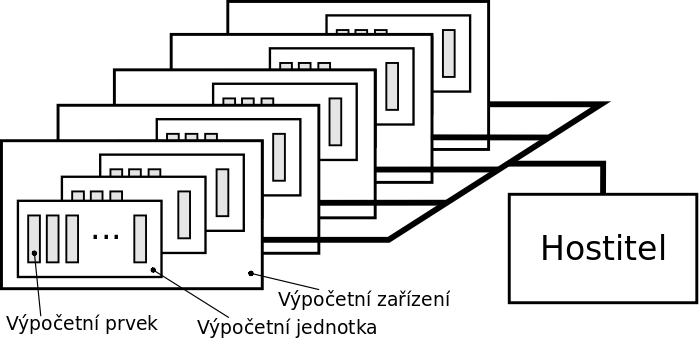
\includegraphics{fig/opencl_platform_model}
	}
    \end{center}
    \caption{Model OpenCL platformy \cite{Khronos:2015}}
    \label{platform}
\end{figure}
\subsubsection{Model proveden�}
Jak ji� bylo zm�n�no aplikace se d�l� na dv� ��sti. Zde hovo��me o~kernelech a~o~hostitelov�
programu, p�i�em� kernel je ten, kdo prov�d� v�po�ty. Tato \uv{pr�ce} je prov�d�na pomoc�
pracovn�ch polo�ek ({\it work-item}) jen� m��eme sdru�ovat do pracovn�ch skupin ({\it
work-group}).

 Hostitel m� za �kol spravovat kontext aplikace a~na jeho z�klad� nastavit prost�ed�, ve
kter�m bude kernel prov�d�t operace. V~prost�ed� mus�me specifikovat a~nastavit tyto polo�ky:
\begin{itemize}
    \item Za��zen� -- jedno a~v�ce za��zen� ovladateln�ch platformou OpenCL.
    \item Objekty kernelu -- OpenCL funkce s~p�ednastaven�mi argumenty podle vybran�ho
        za��zen�.
    \item Objekty programu -- zdrojov� k�d a~jeho spustiteln� verze, kter� implementuj�
        kernely.
    \item Objekty pam�ti -- prom�nn�, ke kter�m m��e p�istupovat hostitel i~OpenCL za��zen�.
	Instance kernel� b�hem sv�ho prov�d�n� operuj� s~t�mito objekty.
\end{itemize}
Hostitel se za��zen�m komunikuje pomoc� front p��kaz�, do nich� se p��kazy roz�ad� podle
typu operace. Jednotliv� p��kazy ve front� se prov�d� relativn� k~ostatn�m p��kaz�m. Po�ad�
prov�d�n� m��e b�t definov�no n�sleduj�c�mi modely:
\begin{itemize}
    \item {\it In-order} -- p��kazy se prov�d� a~maj� efekt tak, jak do fronty p�i�ly.
    \item {\it Out-of-order} -- po�ad� proveden� p��kaz� je omezeno pouze explicitn� uveden�mi
        synchroniza�n�mi body nebo explicitn� definovan�mi z�vislostmi na ud�lostech.
\end{itemize}

\subsubsection{Model pam�ti}
Pr�ce s~pam�t� v~OpenCL se zna�n� li�� od klasick�ho p��stupu, kter� zn�me ze standardn�ch
aplikac� ur�en�ch pro b�h pouze na CPU. Pam�ov� model OpenCL popisuje obsah, strukturu a~chov�n�
pam�ti pou��van� v~platform� vytvo�en� t�mto frameworkem.

 Pro ka�dou aplikaci je t�eba p�esn� definovat, jak p�esn� bude jej� pam� vypadat.
Model d�l�me na �ty�i ��sti:
\begin{itemize}
    \item {\it Oblasti pam�ti} -- definuje, se kter�mi oblastmi pam�ti hostitel a~za��zen� ve
	stejn�m kontextu mohou pracovat.
    \item {\it Objekty pam�ti} -- jsou definovan� v~OpenCL API, o~spr�vu se star� hostitel i
	za��zen�.
    \item {\it Sd�lenou virtu�ln� pam�} -- jedn� se o~virtu�ln� adresov� prostor p��stupn� ob�ma
	��stem aplikace.
    \item {\it Model konzistence} -- definuje pravidla pro oblasti pam�ti, kter� jsou pou��van�
	v�ce jednotkami nar�z a~zaru�uje, �e je dodr�eno po�ad� operac� s~pam�t� a~�e jsou data po
	celou dobu validn�. Takt� definuje synchronizaci nad t�mito oblastmi.
\end{itemize}
Pro n�s je nejd�le�it�j�� pochopit, jak je pam� strukturov�na a~jak na sebe navazuj�
jednotliv� oblasti. To je nejl�pe patrn� z~obr�zku \ref{memory}. Popis struktury:
\begin{itemize}
    \item pam� hostitele (RAM apod.),
    \item pam� za��zen�,
    \begin{itemize}
	\item {\it glob�ln� pam�} -- oblast je p��stupn� pro �ten� i~z�pis v�em jednotk�m
v~kontextu nez�visle na za��zen�,
	\item {\it pam� konstant} -- p�ed zah�jen�m v�po�tu je alokovan� a~inicializov�na
	    hostitelem a~v~pr�b�hu v�po�tu se tato oblast nem�n� v�po�tu,
	\item {\it lok�ln� pam�} -- oblast je p��stupn� v�em pracovn�m polo�k�m ve
	    stejn� pracovn� skupin�,
	\item {\it soukrom� pam�} -- oblast je p��stupn� pouze jedn� pracovn� polo�ce.
    \end{itemize}
\end{itemize}
\begin{figure}[ht]
    \begin{center}
	\scalebox{0.3}{
	    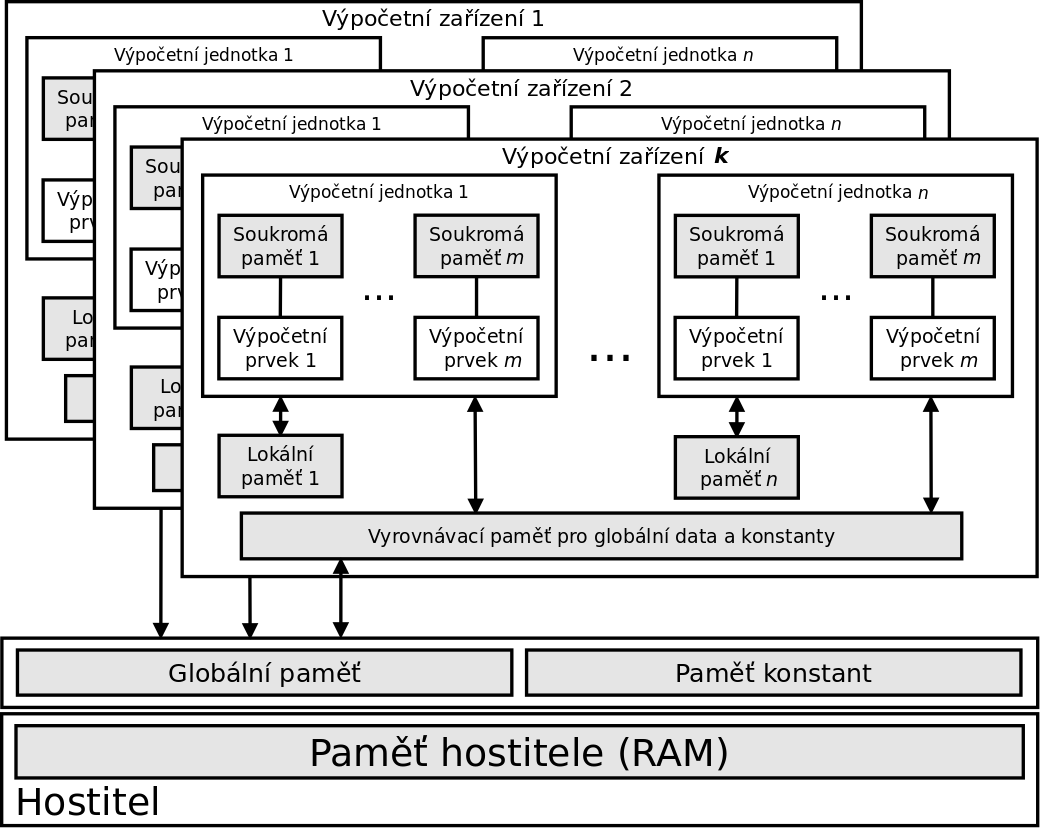
\includegraphics{fig/opencl_memory_structure}
	}
    \end{center}
    \caption{Struktura pam�ti OpenCL \cite{Khronos:2015}}
    \label{memory}
\end{figure}
\subsubsection{Programovac� model}
Tento model lze tak� nazvat jako OpenCL framework. Framework se skl�d� ze t�ech komponent�. Zde za
zm�nku stoj� OpenCL kompil�tor. Ten podporuje pokro�il� jazyk SPIR-V a~jazyk OpenCL C. Dal��
jazyky mohou b�t podporov�ny n�kter�mi implementacemi kompil�toru.


\chapter{N�stroj Wrathion}
\label{ch:wrathion}
Jedn� se o~n�stroj vytvo�en� Janem Shmiedem v~roce 2014 v~r�mci jeho diplomov�
pr�ce~\cite{Schmied}. N�stroj byl vytvo�en pro pou�it� v~projektu {\it Modern� prost�edky pro 
boj s~kybernetickou kriminalitou na Internetu nov� generace, MV, VG20102015022}.
\section{Hlavn� ��sti Wrathionu}
N�stroj slou�� ke obnovov�n� hesel pomoc� brute-force �tok� na tato hesla. Skl�d� se ze t��
��st�:
\begin{itemize}
	\item j�dra -- zprost�edkov�vaj�c�ho funkcionalitu pot�ebnou pro crackov�n�,
	\item modul� -- skrze kter� je zaji�t�na podpora crackov�n� r�zn�ch form�t�,
	\item aplikace -- umo��uj�c� pracovat s~frameworkem a~moduly pomoc� CLI rozhran�.
\end{itemize}
\begin{figure}[ht]
    \begin{center}
	\scalebox{0.34}{
	    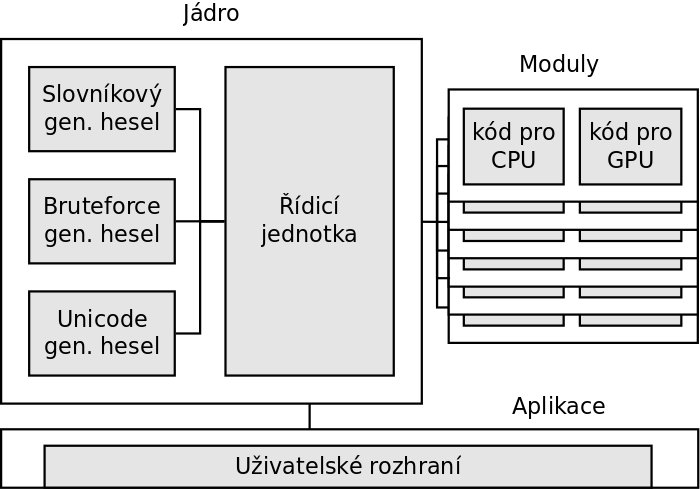
\includegraphics{fig/wrathion_structure}
	}
    \end{center}
    \caption{Sch�ma struktury n�stroje Wrathion \cite{Hranicky}}
    \label{memory}
\end{figure}
\subsection{Gener�tory hesel}
Prvn� ��st� Wrathionu, kterou si rozebereme jsou gener�tory hesel pro �toky. Jedn� se o~esenci�ln�
funkcionalitu. Bez vygenerovan�ch hesel nem��eme na �toky v�bec myslet. V~n�stroji jsou moment�ln�
implementov�ny t�i typy gener�tor�:
\begin{itemize}
    \item {\it Brute-force} -- postupn� generuje v�echny mo�n� permutace ze zadan�ch znak�.
    \item {\it Unicode} -- jedn� se o~upraven� brute-force gener�tor. V~tomto p��pad� je nastavena
	vstupn� abeceda na v�echny Unicode znaky a~z~nich jsou generov�ny mo�n� permutace hesel.
    \item {\it Rule-based} -- velmi podobn� p�edchoz�m variant�m ov�em umo��uje specifikovat r�zn�
	podp�rn� pravidla pro generov�n� hesel. Nap��klad, �e m� b�t prvn� p�smeno velk�, druh� m�
	b�t 'a' a~�e posledn� 2 znaky jsou ��slice. Toto umo��uje z��en� po�tu permutac� a~tedy
	sni�uje �as pot�ebn� k~vygenerov�n� v�ech jejich variant (tento typ gener�toru je teprve
	ve v�voji).
    \item {\it Dictionary} -- slovn�kov� gener�tor, kter� vyu��v� extern� soubory s~�asto
	pou��van�mi hesly.
\end{itemize}
Nej�ast�ji pou��van�m gener�torem je brute-force, kter� je ov�em v�po�etn� n�ro�n�. Jedn� se
v�ak o~snadno paralelizovateln� gener�tor, proto je p��hodn� implementov�n i~jako kernel b��c� na
GPU.
\subsection{Crackery}
Druhou ��st� jsou samotn� crackery, kter� d�l�me podle toho, kdo prov�d� generov�n� hesel a
kdo prov�d� porovn�v�n� hesel:
\subsubsection{CPU cracker}
Zde se standardn� spust� ji� p�edkompilovan� cracker napsan� v~C++ (viz. Obr�zek \ref{CPU}). Nen�
zde ��dn� v�t�� probl�m s~generov�n�m ani n�sledn�m ov��ov�n�m hesel, ov�em v�po�etn� s�la
u~paralelizovateln�ch algoritm� nen� CPU ani zdaleka tak vysok� jako na GPU. Proto, pokud je to
mo�n�, vol�me druhou variantu crackeru.
\begin{figure}[ht]
    \begin{center}
	\scalebox{0.3}{
	    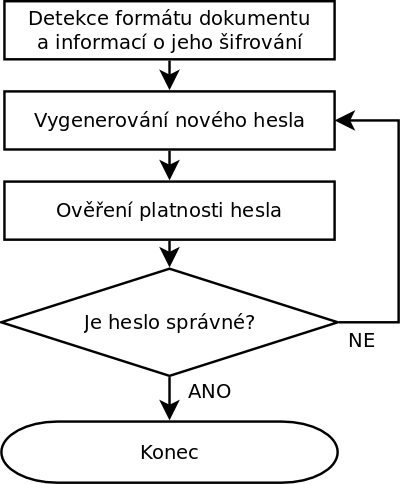
\includegraphics{fig/proces}
	}
    \end{center}
    \caption{Proces generov�n� a~ov��ov�n� hesel na CPU \cite{Schmied}}
    \label{CPU}
\end{figure}

\subsubsection{GPU cracker}
Cracker m��e pracovat ve dvou re�imech (viz. Obr�zek \ref{CPUGPU}). V~prvn�m hesla generujeme na
CPU a~pak je pos�l�me do pam�ti GPU, kde jsou crackerem zpracov�na. To m� ov�em velkou nev�hodu
v~tom, �e mus�me po��d pos�lat data z~pam�ti hostitele (CPU) do priv�tn� pam�ti v�po�etn�ho prvku
(v�po�etn� jednotka na GPU).
\begin{figure}[ht]
    \begin{center}
	\scalebox{0.32}{
	    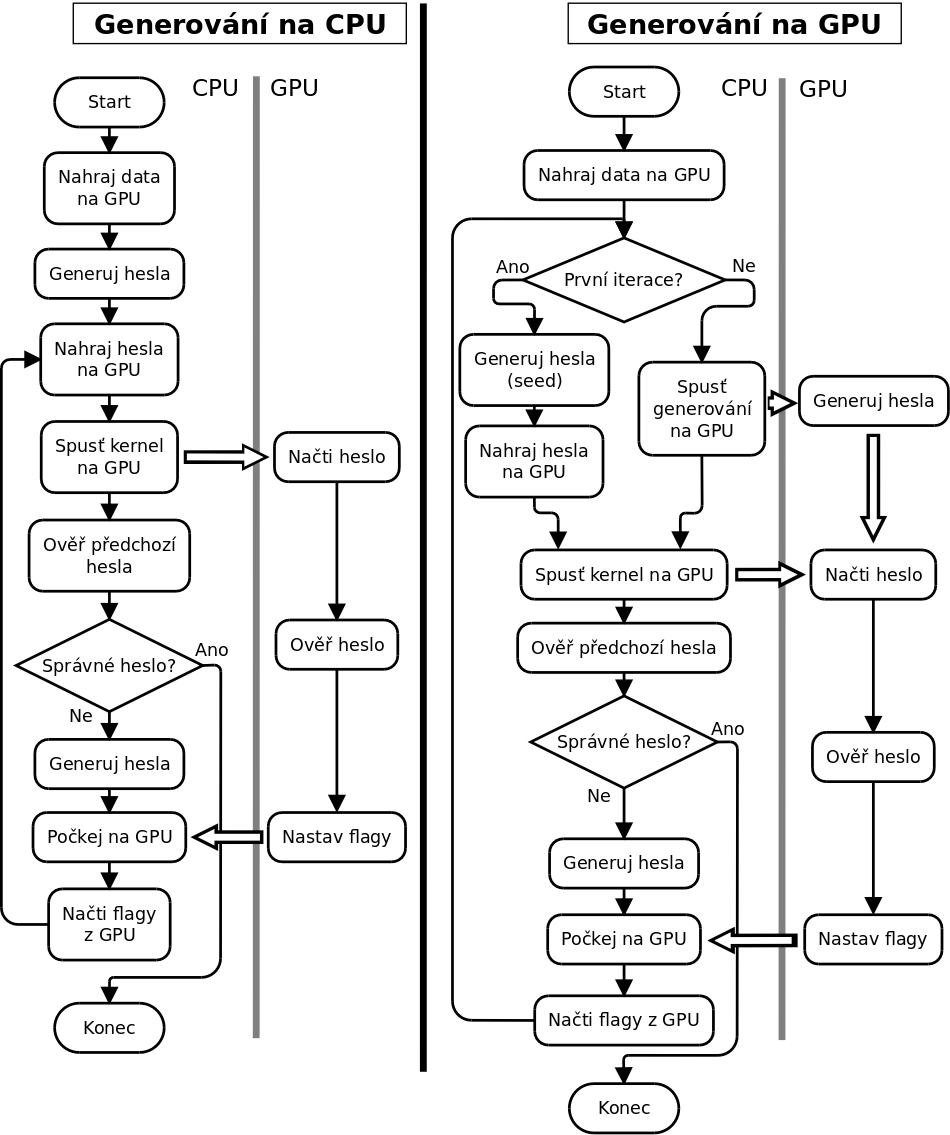
\includegraphics{fig/generators}
	}
    \end{center}
    \caption{Proces generov�n� hesel na CPU a~ov��ov�n� na GPU \cite{Schmied}}
    \label{CPUGPU}
\end{figure}

 Druhou a~efektivn�j�� mo�nost� je generovat hesla p��mo na GPU do priv�tn�ch pam�t� ��m
minimalizujeme mno�stv� dat, kter� mus� putovat od hostitele k~za��zen�. T�mto sn���me v�slednou
prodlevu v�po�t�.

 V~obou p��padech je nutn� p�ed zah�jen�m jak�chkoliv operac� GPU
 inicializovat\linebreak OpenCL syst�m. Tedy vytvo�it kontext, fronty p��kaz�, zajistit na�ten� a
 p�elo�en� po�adovan�ho kernelu a~a� pot� nahr�t nebo vygenerovat data do/na GPU.

\subsection{Moduly}
N�stroj je navr�en s~velk�m d�razem na modularitu. V~sou�asn� dob� obsahuje pouze t�i moduly.
Dal�� moduly pro Wrathion jsou ve f�zi v�voje.

\subsubsection{Modul ZIP}
V~t�to pr�ci n�s nejv�ce zaj�m� modul ZIP. Ten v~p�vodn�m n�vrhu obsahuje pouze �ifrov�n�
obnovov�n� hesel z~archiv� �ifrovan�ch algoritmy PKZIP, AES-128, AES-192, AES-256, co� zanech�v�
prostor pro implementaci dal��ch, form�tem {\it .ZIP}, podporovan�ch metod. Zaj�mavost� je, �e
tento modul byl schopn� v~dob� sv�ho vzniku obnovit heslo �ifrovan�ch {\it .DOCX} soubor�, av�ak
tento nedostatek u~zabezpe�en� form�tu {\it .DOCX} byl pozd�ji odstran�n a~tento modul ji� tedy
nen� schopen obnovit heslo u~soubor� vytvo�en�ch po zm�n�n� aktualizaci.

\subsubsection{Modul DOC}
Dal�� modul pracuje s~form�tem {\it .DOC}, kter� byl pokl�d�n za z�kladn� form�t aplikace MS Word
z~bal�ku MS Office. Tento form�t byl s~p��chodem MS Office 2007 nahrazen form�tem {\it .DOCX}.
N�stroj ve sv� p�vodn� podob� obsahuje pouze podporu pro {\it .DOC} form�t. Tvorba modul� pro
nov�j�� form�t {\it .DOCX} spolu s~form�ty pou��van�mi v~jin�ch aplikac�ch bal�ku MS Office je ve
f�zi v�voje.

\subsubsection{Modul PDF}
Prozat�m posledn� vytvo�en� modul pracuje s~form�tem {\it .PDF}. Zde jsou ji� implementov�ny
bezpe�nostn� revize 1-5. N�stroj po��t� i~s~implementac� revize 6. V�voj t�to funkcionality m��e
b�t zapo�at a� po zve�ejn�n� specifikace t�to revize.

\chapter{Anal�za form�t� .ZIP a~.7z}
\label{ch:formaty}
\section{Form�t .ZIP}
Jedn� se o~jeden z~prvn�ch form�t� souborov�ch archiv�, kter� podporoval kompresi dat. V~roce 1989
vytvo�il Phil Katz program PKZIP v~r�mci n�ho� byl p�edstaven nov� form�t .ZIP. Specifikace
form�tu .ZIP byla publikov�na pod ve�ejnou dom�nou. T�mto krokem pomohl form�tu se st�t
celosv�tov�m otev�en�m standardem~\cite{PKWARE:2015}. V~roce 2015 byl form�t, ve sv� specifikaci
6.3.3 z~roku 2012, p�ijat Mezin�rodn� organizac� pro normalizaci (ISO) a~Mezin�rodn�
elektrotechnickou komis� (IEC) jako�to standard definovan� dokumentem ISO/IEC
21320-1:2015~\cite{ISOIEC:2015}.

 Form�t podporuje velk� mno�stv� r�zn�ch komprima�n�ch algoritm�: Store(bez komprese),
UnShrinking, Expanding, Imploding, Tokenizing, Deflating, Enhanced Deflating, BZIP2, LZMA, WavPack
a PPMd~\cite{PKWARE:2014}. 

 Obdobn� je to i~s~podporou r�zn�ch �ifrovac�ch algoritm�:
\begin{itemize}
    \item {\it PKWARE �ifrov�n�} -- prvotn� �ifrov�n�,
    \item {\it DES, 3DES(112-bit a~168-bit)} -- podporov�no od verze 5.0 z~roku 2002,
    \item {\it RC2 (40-bit, 64-bit a~168-bit)} -- podporov�no od verze 5.0 z~roku 2002,
    \item {\it RC4 (40-bit, 64-bit a~168-bit)} -- podporov�no od verze 5.0 z~roku 2002,
    \item {\it AES (128-bit, 192-bit a~256-bit)} -- podporov�no od verze 5.2 z~roku 2003.
\end{itemize}
Nast�v� zde ale probl�m, �e ��dn� z~a� u� voln� dostupn�ch nebo komer�n�ch n�stroj�
neumo��uje vytvo�en� archiv� se �ifrov�n�m DES, RC2 a~RC4. Z~toho tedy plyne, �e pravd�podobnost
v�skytu archiv� �ifrovan�ch t�mito metodami je minim�ln� respektive t�m�� nulov�.

\subsection{Struktura souboru}
\label{ssec:zip_struct}
Archivy jsou soubory obsahuj�c� dal�� soubory. D� se tedy ��ct, �e se jedn�
o~jak�si\linebreak\uv{schr�nky}, do nich� lze vkl�dat, ale i~vyb�rat, ur�it� soubory r�zn�ch typ�.
U~form�tu .ZIP lze do archiv� nav�c ukl�dat i~adres��e a~tak ukl�dat
cel� struktury tvo�en� z~adres��� a~soubor� \ref{zipstruct}.
\begin{figure}[ht]
    \begin{center}
	\scalebox{0.225}{
	    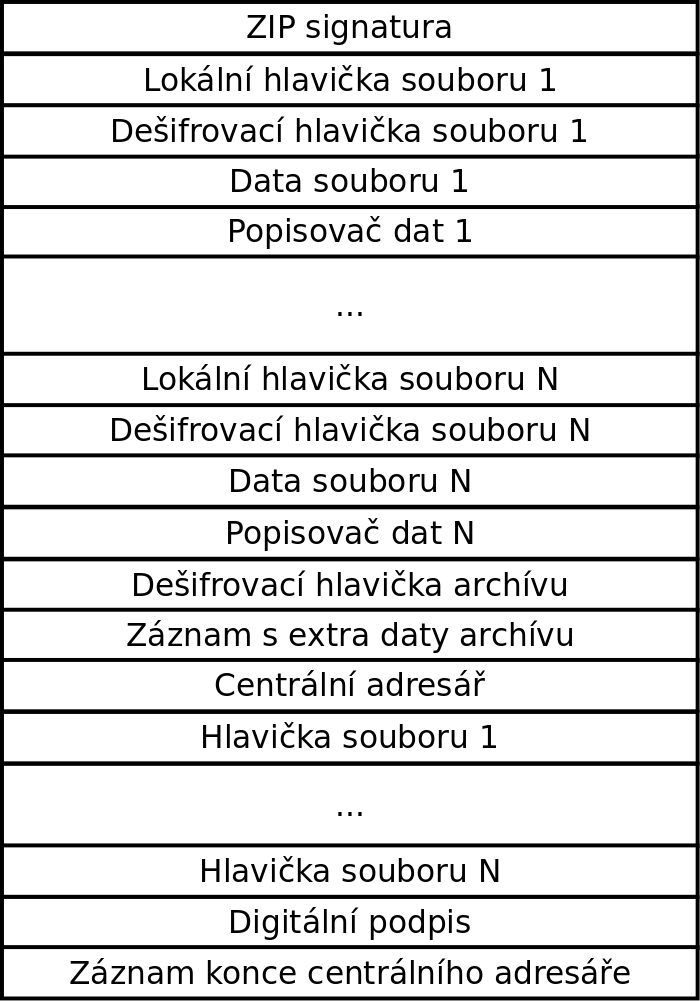
\includegraphics{fig/zip_structure}
	}
    \end{center}
    \caption{Struktura .ZIP souboru \cite{PKWARE:2014}}
    \label{zipstruct}
\end{figure}

 Obsah souboru archivu lze pro lep�� orientaci rozd�lit na ��st obsahuj�c� definice a~data
ulo�en�ch soubor� a~na ��st reprezentuj�c� organizaci adres��� a~soubor�.
\begin{itemize}
    \item Prvn� ��st obsahuje z�znamy, jen� se opakuj� pro ka�d� ulo�en� soubor. Jeden takov�to
z�znam mus� obsahovat alespo� lok�ln� hlavi�ku souboru a~data souboru. Pokud je nastaven
3. bit polo�ky {\it General purpose bit flag} v~lok�ln� hlavi�ce souboru tak mus�me je�t� po��tat
s~t�m, �e za data byla p�id�na sekce {\it Data description} o~velikosti 12 bajt�.
    \item Druh� ��st se skl�d� ze struktury hlavi�ek centr�ln�ho adres��e (Central Directory
Header). Po�et t�chto hlavi�ek odpov�d� po�tu adres��� a~soubor� obsa�en�ch v~tomto
archivu. Hlavi�ka centr�ln�ho adres��e za��n� signaturou [0x50, 0x4b, 0x01, 0x02], podle kter� je
v~souboru identifikovateln� za��tek hlavi�ky. Za n� n�sleduj� metadata souboru. Nap�.: datum a~�as
posledn� �pravy obsa�en�ho souboru, velikost p�ed a~po kompresi atd. Tato struktura hlavi�ek je
ukon�ena z�znamem konec centr�ln�ho adres��e. Ten za��n� signaturou [0x50, 0x4b, 0x05, 0x06]
a~obsahuje informace o~tom na kter�m disku je soubor ulo�en, na kter�m disku za��n� struktura
centr�ln�ho adres��e a~dal��.
\end{itemize}
Od verze form�tu 6.2 jsou p�ed hlavi�kou centr�ln�ho adres��e dal�� polo�ky a~to hlavi�ka
pro de�ifrov�n� archivu a~z�znam o~extra datech archivu. Tyto polo�ky byly p�id�ny
v~z�vislosti na p�id�n� nov� funkce pro �ifrov�n� obsahu hlavi�ek centr�ln�ho adres��e.

\subsubsection{��d�c� struktury definuj�c� �ifrov�n�}
 Zat�m jsme se bavili pouze o~z�kladn� struktu�e archivu. N�s ale sp��e zaj�maj� struktury
archiv�, jen� obsahuj� soubory v~za�ifrovan� podob�. Zda je soubor �ifrov�n lze zjistit z~jeho
lok�ln� hlavi�ky nebo z~jeho hlavi�ky centr�ln�ho adres��e a~konkr�tn� z~prvn�ho a~sedm�ho bitu
polo�ky {\it General Purpose Bit Flag}. Nastaven� prvn�ho bitu indikuje, �e je soubor �ifrov�n.
\begin{itemize}
    \item Pokud plat�, �e nen� z�rove� nastaven i~sedm� bit, je za lok�ln� hlavi�ku souboru
        p�id�na hlavi�ka �ifrov�n�. Hlavi�ka �ifrov�n� se v�e pouze k~�ifrov�n� pomoc� tradi�n�
        metody od spole�nosti PKWARE.
    \item Pokud je nastaven i~sedm� bit indikuj�c� pou�it� takzvan�ho \uv{siln�ho
	�ifrov�n�}, hlavi�ka �ifrov�n� se negeneruje, ale p�id�vaj� se informace o~�ifrov�n� do
        hlavi�ky centr�ln�ho adres��e a~generuje se z�znam s~hlavi�kou pro de�ifrov�n�, jeho�
	��st se tv��� jako sou��st dat souboru a~nach�z� se na sam�m po��tku �ifrovan�ch dat
	souboru.
\end{itemize}
Informace o~metod� �ifrov�n�, d�lce kl��e atd., jsou uvedeny v~druh� ��sti souboru
z~d�vod� vy��� bezpe�nosti. P�esn�ji v~polo�ce {\it Extra Fields} v~hlavi�ce centr�ln�ho adres��e
p��slu��c� souboru. Polo�ku {\it Extra Fields}, pozn�me podle jej� signatury, kterou za��n� a~m�
hodnotu [0x00, 0x17]. Dal�� polo�ky obsahuj� informace o~pou�it�m �ifrovac�m algoritmu, d�lce
kl��e pro �ifrov�n� a~pole p��znak� {\it Flags} definuj�c�, zda je archiv �ifrovan�, jak� je
pou�ita kompresn� metoda, co je vy�adov�no pro de�ifrov�n�, zda je vy�adov�no pouze heslo nebo
pouze certifik�t nebo je mo�n� pou��t bu� heslo, nebo certifik�t. Dal�� mo�nosti z�vis� na pou�it�m
certifik�tu.

 Z�znam pro de�ifrov�n� obsahuje o~inicializa�n� vektor (IV, s�l), identifik�tor algoritmu pro
de�ifrov�n�, bitovou d�lku �ifrovac�ho kl��e, za�ifrovan� vzorek n�hodn�ch dat (Erddata) a~hlavn�
o~informace pro validaci hesla (VData) a~CRC-32 (VCRC32)\footnote{{\it Cyclic Redundancy Code} -
speci�ln� he�ovac� funkce slou��c� pro detekci chyb / zm�n dat oproti p�vodn� hodnot�} t�chto
valida�n�ch dat. 



\section{Form�t .7z}
\label{sec:7z}
Vznik tohoto form�tu se datuje do roku 1999 a~jeho autorem je Igor Pavlov. Stejn� jako aplikace
7-Zip a~n�stroj� spojen�ch s~t�mto form�tem (7-Max, 7-Benchamark). Form�t takt� slou��
k~vytvo�en� souborov�ch archiv� podobn� jako .ZIP. Form�t se proslavil hlavn� svoj� otev�enost� a
modul�rn� strukturou. Ta umo��uje skl�d�n� libovoln�ch kompresn�ch, konverzn�ch a~�ifrovac�ch
metod.

 Mezi podporovan� kompresn� metody se �ad� LZMA, LZMA2, PPMD, BCJ, BCJ2, BZip2 a
Deflate. Jako v�choz� metoda je br�na LZMA. Hlavn� v�hody t�to metody jsou~\cite{7z:2015}:
\begin{itemize}
    \item vysok� kompresn� koeficient,
    \item prom�nn� velikost slovn�ku,
    \item mal� n�roky na pam� p�i dekompresi,
    \item podpora zpracov�n� pomoc� multi-threading a~hyper-threading.
\end{itemize}
Dal�� v�hodou form�tu je podpora komprese velk�ch soubor�, n�zvy soubor� v~Unicode
k�dov�n�, mo�nost spojen� v�ce soubor� do jednoho toku, kter� je pak teprve komprimov�n, komprese
a �ifrov�n� hlavi�ek archiv� a~dal��.

 Standardn� pou�itou �ifrovac� metodou je AES-256 vy�aduj�c� 256-bitov� �ifrovac� heslo.
Takov�to heslo se vytv��� pomoc� he�ovac� funkce SHA-256 z~u�ivatelem zadan�ho hesla. Pro je�t�
vy��� zabezpe�en� je provedeno \(2^{19}\) iterac� p�i ka�d�m vytv��en� hesla. To m��e m�t na
slab��ch za��zen�ch za n�sledek znatelnou prodlevu, ne� za�ne komprese soubor� a~�ifrov�n�.

\subsection{Struktura souboru}
\label{ssec:7z_struct}
Nepr�zdn� soubor tohoto form�tu m� �ty�i ��sti, kter� v~n�m mus� b�t obsa�eny viz.
\ref{7zstruct}. Jedn� se o~polo�ky: 
\begin{itemize}
    \item Prvn� ��st se nach�z� hned za��tku souboru a~jedn� se o~hlavi�ku se signaturou ({\it
	7zSignature}) ['7', 'z', 0xBC, 0xAF, 0x27, 0x1C] definuj�c� za��tek souboru dan�ho typu.
	Za n� v~r�mci stejn� hlavi�ky jsou informace o~verzi archivu, CRC hlavi�ky a~jako posledn�
	jsou polo�ky t�kaj�c� se pozice n�sleduj�c� hlavi�ky. Najdeme zde relativn� adresu
	(uvedena jako vzd�lenost od konce �vodn� hlavi�ky), n�sleduje pak d�lka dal�� hlavi�ky a~CRC pro tyto dv� polo�ky.
    \item Druh� ��st obsahuje zpracovan� data vytvo�en�ch proud�, tedy data samostatn�ch nebo
	p��padn� i~spojen�ch soubor� po kompresi, �ifrov�n� apod.
    \item T�et� ��st obsahuje zpracovan� informace slou��c� jako podp�rn� data pro hlavi�ku a~jej�
	polo�ky.
    \item Posledn� �tvrt� ��st� je 7z hlavi�ka ({\it 7zHeader}), jej�� za��tek je definov�n
	v~�vodn� hlavi�ce. Tato hlavi�ka m� prom�nnou d�lku a~strukturu. Je ji tedy pot�eba
	proch�zet postupn� a~zji��ovat, kter� polo�ky jsou p��tomny a~kter� ne. K~identifikaci
	jednotliv�ch polo�ek slou�� jednobajtov� identifik�tor zapsan� v~hexadecim�ln� form�.
	Identifik�tory za��naj� hodnotou 0x00 a~kon�� 0x19. M�me tedy k~dispozici 25 polo�ek
	s~r�znou velikost�, strukturou a~polo�kami. Jedin�mi povinn�mi �daji v~hlavi�ce jsou
	polo�ky zna��c� za��tek hlavi�ky (0x01) a~konec hlavi�ky (0x00). V�echny ostatn� polo�ky
	jsou p��padn� um�st�ny mezi n� a~za��naj� p��slu�n�m identifik�torem~\cite{Pavlov:2010}.  
\end{itemize}
\begin{figure}[ht]
    \begin{center}
	\scalebox{0.35}{
	    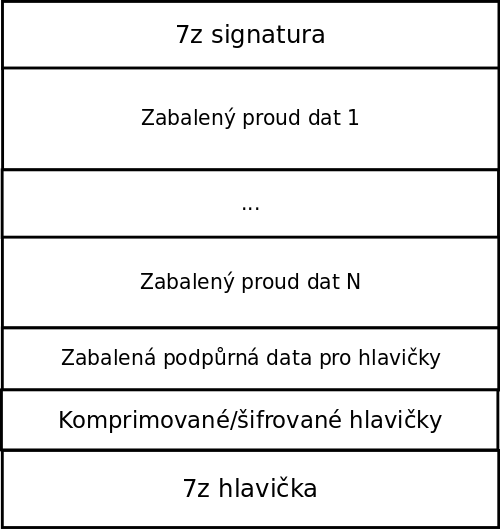
\includegraphics{fig/7z_structure}
	}
    \end{center}
    \caption{Struktura .7z souboru \cite{Pavlov:2015}}
    \label{7zstruct}
\end{figure}
Pro ��ely t�to pr�ce n�s p�edev��m zaj�m� hlavi�ka {\it 7zHeader} a~v~n� obsahy polo�ek nesouc�ch
informace o~proudech dat (0x03 nebo 0x04). V~nich konkr�tn� polo�ka informace o~k�derech (0x07),
ve kter� se mus�me propracovat k~poli bajt� {\it CodecInfo}. Hodnoty tohoto pole mus�me otestovat
a zjistit, zda se shoduj� s~identifik�torem standardn� �ifrovac� metody AES-256 + SHA-256
[0x06, 0xF1, 0x07, 0x01]~\cite{Pavlov:2015}.

\section{Srovn�n�}
Pokud budeme srovn�vat form�ty z~pohledu komprese, zjist�me, �e .7z je dle m��en� efektivn�j��
ne�
.ZIP\footnote{\url{http://www.howtogeek.com/200698/benchmarked-whats-the-best-file-compression-format/}}. Ov�em n�s sp��e zaj�m� zabezpe�en�.

 �ifrov�n� form�tu .ZIP metodou PKZIP nem� smysl ani porovn�vat s~ostatn�mi, nebo� se jedn�
o~metodu, kter� ji� nedosta�uje dne�n�m bezpe�nostn�m standard�m~\cite{PKWARE:2014}. 

 Pokud se ale pod�v�me na siln�j�� metody zabezpe�en�, zjist�me, �e form�ty jsou z~hlediska
bezpe�nosti vyrovnan�. Oba dva podporuj� AES-256 s~vyu�it�m n�jak� he�ovac� metody pro zabezpe�en�
hesla. Oba form�ty tak� podporuj� �ifrov�n� hlavi�ek obsahuj�c�ch informace o~metod�ch, kter� jsou
pou��v�ny a~jak� soubory obsahuj�.

 Form�t .ZIP p�ekon�v� .7z mo�nost� pou�it� elektronick�ch podpis� (certifik�t typu X.509v3)
 k~�ifrov�n� soubor� nam�sto hesel. 7z tuto funkcionalitu v�bec neobshahuje. 


\chapter{N�vrh modul�}
\label{ch:moduly}
V~t�to kapitole se pod�v�me na to, jak z~v��e popsan�ch algoritm�, technologi� a~struktur�ln�ch
anal�z archiv� vytvo��me roz�i�uj�c� moduly pro n�stroj Wrathion. Tato kapitola si klade za c�l
obecn� popsat, jak se budou soubory jednotliv�ch form�t� proch�zet. Tedy jak� data se z~nich budou
��st, jak� operace je pot�eba prov�st nad vygenerovan�mi hesly a~jak se bude prov�d�t ov��ov�n�
shody hesel.

\section{Modul ZIP}
Jako prvn� si nast�n�me modul ZIP. Nemus�me zde �e�it n�vrh cel�ho modulu a~v�ech
mo�nost� pro form�t, ale pouze roz���en� funkcionality o~zat�m nepodporavan� metody zabezpe�en�.

 Moment�ln� verze ZIP modulu podporuje pouze star� �ifrov�n� PKWARE a~�ifrov�n� AES. Podpora
�ifrov�n� AES je v�ak ne�pln�. Modul moment�ln� podporuje pouze speci�ln� verzi AES, je� si
vytvo�ili v�voj��i n�stroje WinZip. Ti si vytvo�ili vlastn� o�ezanou AES hlavi�ku a~ozna�ili
soubor vlastn� metodou. Existuj� ov�em n�stroje jako SecureZIP od firmy PKWARE umo��uj�c� tak�
za�ifrovat obsah archiv� pomoc� �ifrovac� metody AES, s~n�� si sou�asn� modul i~p�es podporu
zji�t�n� hesla pro AES neporad�.

 Dal�� �ifrovac� metodou, kterou nab�z� n�stroj SecureZIP je 3DES. S~n�m si moment�ln� verze
neporad� v�bec a~je tedy vhodn� tuto funkcionalitu doplnit.

\subsubsection{Zji�t�n� informac� z~archivu}
N�sleduj�c� text popisuje postup z�sk�v�n� a~zpracov�n� informac� nutn�ch pro rozhodnut�, zda se
jedn� o~ZIP soubor, zda je soubor �ifrov�n, jakou metodou je �ifrov�n, jak� jsou inicializa�n�
hodnoty pou�it� p�i �ifrov�n� apod. To v�e je pot�eba pro roz���en� funkcionality modulu. Popis se
prim�rn� nesoust�ed� na z�sk�n� dat pro ji� implementovan� funkce, ale pouze dat d�le�it�ch pro
roz���en� funkcionality modulu (detailn� popis hlavi�ek a~hodnot v~nich je v~sekci
\ref{ssec:zip_struct}):
\begin{enumerate}
    \item Zji�t�n� signatury -- pod�v�me se na prvn� 4 bajty a~porovn�me je se signaturou [0x50,
	0x4B, 0x03, 0x04]. T�m ov���me, zda se jedn� o~ZIP soubor.
    \item P�e�ten� {\it General purpose bit flag} -- hodnotu p��znak� (flag�) z�sk�me
z~n�kter� z~hlavi�ek\footnote{Lok�ln� hlavi�ka souboru nebo hlavi�ka souboru v~centr�ln�m
	adres��i. Hlavi�ka souboru v~centr�ln�m adres��i obsahuje v�echny polo�ky lok�ln� hlavi�ky
	plus n�jak� nav�c.} prvn�ho souboru.
    \item Anal�za p��znak� -- zji��ujeme zda jsou nastaveny prvn� a~sedm� bit p��znak� na hodnotu
	1. Pokud nalezneme �ifrov�n� u~jednoho souboru p�edpokl�d�me, �e v�echny ostatn� soubory
	jsou takt� �ifrovan� a~�e byla pou�ita stejn� �ifrovac� metoda. Pokud je nastaven i~13.
	bit mus�me prov�st �ten� de�ifrovac� hlavi�ky archivu a~pomoc� n� de�ifrovat celou
	strukturu centr�ln�ho adres��e. Postup de�ifrov�n� je identick� s~de�ifrov�n�m soubor�.
    \item P�e�ten� {\it Compression method} -- z~n�kter� z~hlavi�ek %\footnotemark[\value{footnote}] 
	souboru. Tato polo�ka n�s zaj�m�, pouze pokud byly bity jedna a~sedm p��znak� nastaveny na
	hodnotu 1. ��slo uveden� v~t�to polo�ce n�m dovoluje zjistit, zda byla pou�ita �ifrovac�
	metoda WinZip AES (hodnota 99). Pou�it� jin� hodnoty indikuje pou�it� n�kter� z~dal��ch
	�ifrovac�ch metod definovan�ch ve specifikaci form�tu .ZIP~\cite{PKWARE:2014}.
    \item P�e�ten� {\it Extra fields} -- pot�ebujeme naj�t hlavi�ku s~daty o~�ifrov�n�, kter� se
	m��e vyskytnout pouze za hlavi�kou souboru v~centr�ln�m adres��i. V~tomto kroku zjist�me
	informace o~pou�it� �ifrovac� metod�, d�lce kl��e atd.
    \item Z�sk�n� hodnot hlavi�ky pro de�ifrov�n� -- nach�z� se p�ed ulo�en�mi daty souboru.
	Pot�ebujeme z�skat pou�it� inicializa�n� data pot�ebn� pro �ifrovac� s~de�ifrovac� funkce.
	A~tak� data pro ov��en� hesla v�etn� jejich kontroln�ho sou�tu (CRC32).
\end{enumerate}
Jakmile takto z�sk�me v�echna pot�ebn� data, p�esuneme se k~hled�n� pou�it�ho hesla. Tento proces
bude mo�n� realizovat za vyu�it� CPU nebo GPU. Pro ob� tato za��zen� je nutn� vytvo�it samostatn�
k�d. K�d pro CPU �ist� v~jazyce C++ s~mo�nost� vyu�it� n�kter�ch ji� implementovan�ch funkc� a
gener�tor� obsa�en�ch v~n�stroji Wrathion. Pro GPU je t�eba vytvo�it k�d v~C++, kter� pob�� na
CPU a~bude inicializavat GPU a~rozd�lovat pr�ci pracovn�m jednotk�m na n� um�st�n�ch a~pot� kernel
v~OpenCL pro implementov�n� kernelu, kter� pob�� na pracovn�ch jednotk�ch. Av�ak v~obou
p��padech p�jde o~toto�n� Algoritmus \ref{alg:zip_ver}.

\begin{algorithm}[ht]
    \SetStartEndCondition{ (}{)}{)}\SetAlgoBlockMarkers{}{}%
    \SetKwFor{For}{for}{\string:}{}%
    \SetKwIF{If}{ElseIf}{Else}{if}{}{else if}{else}{}%
    \SetKwRepeat{Repeat}{repeat}{until}%
    \SetKwInOut{Input}{vstup}\SetKwInOut{Output}{v�stup}
    \AlgoDisplayBlockMarkers\SetAlgoNoLine%
    \DontPrintSemicolon
    \Input{Data z�skan� z~hlavi�ky pro de�ifrov�n� (IV, Erd, VDlen, Data)}
    \Output{Posledn� vygenerovan� heslo}
    $shoda = FALSE$\;
    \Repeat{$shoda$}{
	heslo = generujHeslo ()\;
	odvozene\_heslo = odvodHeslo (SHA1(heslo))\;
	rd = desifruj (Erd, odvozene\_heslo, IV)\tcc*{Random hodnotu pro �ifrov�n�}
	odvozene\_heslo = odvodHeslo (SHA1(rd + IV))\;
	desifrovana\_data = desifruj (Data, odvozene\_heslo, IV)\;
	presun (Data, VDlen, VData)\tcc*{VDlen bajt� z~Data do VData} 
	VCRC32 = Data\;
	CRC = spocitejCRC32 (VData)\;

	\If{$ CRC ==  VCRC32 $}{
	    $shoda = TRUE$\;
	}
    }
    \caption{Princip ov��en� vygenerovan�ho hesla pro ZIP archiv}\label{alg:zip_ver}
\end{algorithm}



\section{Modul 7z}
V~tomto p��pad� se jedn� o~�pln� nov� modul. Bude tedy pot�eba nadefinovat v�echny struktury
pot�ebn� k~provozu modulu v~r�mci n�stroje Wrathion a~implementovat metody �ifrov�n�, he�ov�n�,
odvozov�n� hesel a~jin� pou��van� form�tem .7z.

\subsubsection{Zji�t�n� informac� z~archivu}
Archiv form�tu .7z v~sob�, stejn� tak jako .ZIP archiv, nese informace nutn� pro umo�n�n�
de�ifrov�n� souboru. V~tomto p��pad� je v�ak o~n�co slo�it�j�� je z�skat. Struktura 7z archivu
je hodn� komplexn� a~prom�nliv�. Struktura hlavi�ek do zna�n� m�ry p�ipom�n� datab�zi. Pro
detailn� porozum�n� struktu�e ��d�c�ch dat form�tu je t�eba nahl�dnout do souboru
7zFormat.txt~\cite{Pavlov:2010}. Pot�ebn� informace lze z�skat n�sleduj�c�m zna�n� zjednodu�en�m
teoretick�m postupem:
\begin{enumerate}
    \item Ov���me signaturu -- jedn� se o~prvn�ich 6 bajt� souboru, kter� mus� odpov�dat hodnot�
v~sekci \ref{ssec:7z_struct}. 
    \item Z�sk�me pozici a~velikost dal�� hlavi�ky -- p�esko��me na pozici 6 bajt� za signaturou
        a~z�sk�me pozici dal�� hlavi�ky. Z~n�sleduj�c� hodnoty z�sk�me d�lku n�sleduj�c� hlavi�ky.
    \item P�ejdeme na dal�� hlavi�ku -- mus�me se pod�vat na signaturu hlavi�ky, pokud odpov�d�
	hodnot� 0x17 mus�me proj�t jej� obsah.
    \item Detekce �ifrov�n� hlavi�ky -- v~hlavi�ce {\it Folders} za��naj�c� signaturou 0x0B,
	nejprve hled�me hodnotu [0x06, 0xF1, 0x07, 0x01]. Jej� n�lez znamen�, �e data hlavi�ky jsou
	�ifrov�na metodou 7zAES.
    \item Z�sk�n� dat pro �ifrov�n� -- v~p��pad� n�lezu �teme data inicializa�n�ho vektoru a~po�et
	iterac� pou�it� he�ovac� funkce pro odvozen� hesla pro �ifrov�n� (defaultn� 19).
    \item De�ifrov�n� hlavi�ky -- de�ifrujeme podle Algoritmu~\ref{alg:7z_desifr}.
    \item Detekce hlavi�ky pro dekompresi -- hled�me ve stejn� sekci jako v~bod� 5. Zde v�ak
	p�tr�me po hodnot� [0x03, 0x01, 0x01] zna��c� pou�it� LZMA pro kompresi.
    \item Provedeme dekompresi hlavi�ky -- pomoc� algoritmu LZMA.
    \item Vypo��t�me CRC dat po dekompresi.
    \item Porovn�me vypo�ten� CRC s~odpov�daj�c�m CRC ulo�en�m v~hlavi�ce {\it Digest}, pokud
	nesouhlas�, vrac�me se na krok 6.
    \item Pro zji�t�n� hesla k~soubor�m se pod�v�me do dekomprimovan�ch dat a~postupujeme od kroku
	4 obdobn�m zp�sobem, av�ak nyn� pracujeme s~daty souvisej�c�mi se soubory nam�sto
        s~hlavi�kou.
\end{enumerate}
\begin{algorithm}[H]
    \SetStartEndCondition{ (}{)}{)}\SetAlgoBlockMarkers{}{}%
    \SetKwFor{For}{for}{\string:}{}%
    \SetKwInOut{Input}{vstup}\SetKwInOut{Output}{v�stup}
    \AlgoDisplayBlockMarkers\SetAlgoNoLine%
    \DontPrintSemicolon
    \Input{Data z�skan� z~hlavi�ky pro de�ifrov�n� (IV, pocet\_iteraci) a~�ifrovan� data}
    \Output{De�ifrovan� data (neov��en�)}
    heslo = generujHeslo ()\;
    retezec = vytvorRetezec(heslo)\tcc{512 * p�r (heslo, 64b ��slo <0,512))}
    \For{$i = 0; i< pocet\_iteraci; i++$}{
	retezec = SHA256 (retezec)\;
    }
    citelna\_data = desifrujData(Data, retezec, IV)\;
    
    \caption{Princip vytvo�en� hesla pro de�ifrov�n� pomoc� 7z}\label{alg:7z_desifr}
\end{algorithm}

\chapter{Z�v�r}
Obs�hnout v�echny mo�nosti a~nastaven� analyzovan�ch form�t� je zna�n� n�ro�n� proces, kter�
ve v�t�in� p��pad� ani nestoj� za n�mahu. D�vodem je n�zk� po�et dostupn�ch n�stroj� schopn�ch tyto
hodnoty nastavit, co� plat� hlavn� pro form�t ZIP.

 Struktury jednotliv�ch form�t� byly pops�ny tak, aby bylo mo�n� chyb�j�c� nebo nejasn� informace
dohledat ve specifikac�ch form�tu a~nebylo nutn� slo�it� hledat, o~jak� hodnoty se jedn�. Zde
je nutno podotknout, �e, jak ji� bylo zm�n�no, struktura 7z souboru je hodn� komplexn� a~prom�nn�.
Bohu�el dokumentace tohoto form�tu je zna�n� nedosta�uj�c� a~je tedy nutn� str�vit hodn� �asu
studiem struktury, zdrojov�ch k�d� a~f�ra v�voj��e pro z�sk�n� dal��ch a~detailn�j��ch informac�.

 N�vrh roz���en� modulu pro ZIP by m�l z~v�t�iny odpov�dat tomu, jak bude roz���en� vypadat po jeho
implementaci. Tak� na z�klad� pr�zkumu v~tomto odv�tv� by roz���en� modul m�l b�t nap�ed p�ed
konkurenc�. N�kter� zn�m� n�stroje toti� maj� podporu pouze pro WinZip AES a~PKWARE �ifrov�n�
(John the Ripper) nebo moment�ln� neposkytuj� funkcionalitu k~form�tu .ZIP (oclHashcat).  

 U~modulu 7z se jedn� sp�� o~teoretick� n�stin, jak by mohl modul vypadat a~jak by
mohly jednotliv� ��sti algoritmu fungovat. N�kter� d�le�it� informace toti� nejsou nikde detailn�
pops�ny. Hled�n� informac� ve zdrojov�ch k�dech 7zip-u je d�ky absenci koment��� a~vysok�
abstrakci k�du zna�n� n�ro�n� a~zdlouhav�. N�vrh modulu bude tedy pot�eba pravd�podobn�
modifikovat na z�klad� informac� zji�t�n�ch b�hem implementace jednotliv�ch ��st� modulu.

 B�hem implementace bude zapot�eb� vytvo�it dv� verze obou modul�. Jednu verzi b��c� pouze na
CPU a~druhou, kter� bude podporovat paraleln� zpracov�n� na GPU. V~n�vaznosti na implementaci
bude pot�eba prov�st m��en� rychlosti a~srovn�n� s~dal��mi n�stroji. Podle v�sledk� srovn�n�
jde odhadnout, jak moc optim�ln� n� modul je a~zda je pot�eba jej upravit a~vyladit nebo
zda je v~r�mci mo�nost� optimalizov�n.

%=========================================================================
 % viz. obsah.tex

  % Pouzita literatura
  % ----------------------------------------------
\ifslovak
  \makeatletter
  \def\@openbib@code{\addcontentsline{toc}{chapter}{Literatúra}}
  \makeatother
  \bibliographystyle{czechiso}
\else
  \ifczech
    \makeatletter
    \def\@openbib@code{\addcontentsline{toc}{chapter}{Literatura}}
    \makeatother
    \bibliographystyle{czechiso}
  \else 
    \makeatletter
    \def\@openbib@code{\addcontentsline{toc}{chapter}{Bibliography}}
    \makeatother
    \bibliographystyle{plain}
  %  \bibliographystyle{alpha}
  \fi
\fi
  \begin{flushleft}
  \bibliography{literatura} % viz. literatura.bib
  \end{flushleft}

  % Prilohy
  % ---------------------------------------------
  \appendix
\ifczech
  \renewcommand{\appendixpagename}{Přílohy}
  \renewcommand{\appendixtocname}{Přílohy}
  \renewcommand{\appendixname}{Příloha}
\fi
\ifslovak
  \renewcommand{\appendixpagename}{Prílohy}
  \renewcommand{\appendixtocname}{Prílohy}
  \renewcommand{\appendixname}{Príloha}
\fi
  \appendixpage

\ifslovak
  \section*{Zoznam príloh}
  \addcontentsline{toc}{section}{Zoznam príloh}
\else
  \ifczech
    \section*{Seznam příloh}
    \addcontentsline{toc}{section}{Seznam příloh}
  \else
    \section*{List of Appendices}
    \addcontentsline{toc}{section}{List of Appendices}
  \fi
\fi
  \startcontents[chapters]
  \printcontents[chapters]{l}{0}{\setcounter{tocdepth}{2}}
  \chapter{Obsah CD}
\chapter{Manual}
%\chapter{Konfigrační soubor}
%\chapter{RelaxNG Schéma konfiguračního soboru}
%\chapter{Plakat}

 % viz. prilohy.tex
\end{document}
